 \documentclass[12pt]{article}
\usepackage[a4paper, margin=.30in]{geometry}

\usepackage{array}
\usepackage{graphicx, subfig, wrapfig, fancyhdr, lastpage }
\newcommand\headerMe[2]{\noindent{}#1\hfill#2}
\usepackage[mathscr]{euscript}



\pagestyle{fancy}
\fancyhf{}

\rfoot{\em{Page \thepage \hspace{1pt} / \pageref{LastPage}}}
\begin{document}

\headerMe{Royaume du Maroc}{année scolaire \emph{2022-2023}}\\
\headerMe{Ministère de l'Éducation nationale, }{  Professeur :\emph{Zakaria Haouzan}}\\
\headerMe{du Préscolaire et des Sports}{Établissement : \emph{Lycée SKHOR qualifiant}}\\

\begin{center}
Devoir  N°3 Semestre 02 \\
   Filière Tronc Commun Scientifique\\
Durée 2h00
\\
    \vspace{.2cm}
\hrulefill
\Large{Chimie 7pts/42min}
\hrulefill\\

    %\emph{Les Trois parties sont indépendantes}
\end{center}
%end Headerss------------------------

\section*{Partie 1 :Transformation chimique d’un système.\dotfill (4pts) }
%__________________Chimie ______________________-
%%%%%%%+_+_+_+_+_+_+_+_+_Partie1
On introduit un morceau d’aluminium $Al_{(S)}$ de masse $m=16,2g$ dans une solution d’acide chlorhydrique $(H^+_{(aq)}+Cl^-_{(aq)})$ de concentration   $C$=$0,24 mol/L$ et de volume $V=1L$. la réaction chimique mise en jeu entre le morceau d’aluminium $Al_{(S)}$ et les ions $H^+_{(aq)}$ produit les ions $Al^{3+}_{(aq)}$ et le dihydrogène gazeux $H_{2(g)}$.

\begin{enumerate}
	\item  Calculer $n_1$ et $n_2$ les quantités de matières initiales respectives de $H^+_{(aq)}$ et de $Al_{(S)}$.\dotfill (0,5pts)

	\item  Ecrire l’équation de la réaction mise en jeu équilibrée puis tracer le tableau d’avancement associé à cette
réaction. \dotfill (0,5pts)
\item  Déterminer $X_{max}$ l’avancement maximal puis déduire le réactif limitant. \dotfill(1pts)
\item  En se basant sur le tableau d’avancement , donner le bilan de matière à l’état final .\dotfill(1pts)
\item  déduire $V_{f(H_2)}$ le volume finale du dihydrogène produit à l’état final.\dotfill(1pt)
\end{enumerate}

\textbf{Données : }La masses molaires $M(Al) = 27g/mol$ et Volume molaire $V_m = 24 L.mol^{-1}$.


\section*{Partie 2 :Les Réactions Chimiques\dotfill (3pts) }

l’équation de la réaction mise en jeu entre les ions argent $Ag^+_{(aq)}$ el le plomb $Pb_{(S)}$ de masse molaire $M(Pb)$=$207g/mol$ s’ecrit comme suit :

$$Pb_{(s)} + 2Ag^+_{(aq)} \rightarrow Pb^{2+}_{(aq)} + Ag_{(s)}$$

\begin{itemize}
	\item la concentration initiale des ions $Ag^+_{(aq)}$ vaut $[Ag^+_{(aq)}]+i=0,8mol/L$ et le volume de la solution qui est le siège de la réaction vaut $V=1L$.
	\item  A l’état final la concentration des ions $Ag^+_{(aq)}$ vaut $[Ag^+_{(aq)}]_f=0,2mol/L$.
\end{itemize}

\begin{enumerate}
	\item  Déterminer $X_{max}$ l’avancement maximal puis déduire le réactif limitant. \dotfill(1pts)
\item  Trouver $m_{i}(Pb)$ la masse initiale du plomb introduit dans la solution. \dotfill(1pts)
\item  Trouver $[Pb^{2+}]_f$ la contraction des ions $Pb^{2+}$ à l’état final. \dotfill(1pts)
\end{enumerate}


%__________________Chimie ______________________-
%%%%%%%+_+_+_+_+_+_+_+_+_Partie1

%_____________________________________PHYSIque Partie 22222____________________________________________________________________________

    %\vspace{2cm}
\hrulefill\\
\begin{center}
\hrulefill
\Large{Physique 13pts/72min}
\hrulefill\\
    \emph{Les deux parties sont indépendantes}
\end{center}
%end Headerss------------------------

%\vspace{3cm}

\hrulefill\\
%_________________partie 2  : gravitation universelle :)


\section*{Partie 2 : Montages électroniques \dotfill(5pts)}

Soit le circuit électrique ci-contre :
\begin{center}
    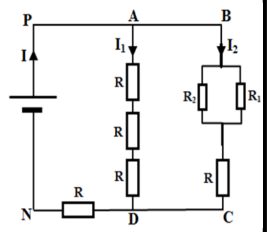
\includegraphics[width=0.32\textwidth]{./img/ex00.png}
\end{center}
\textbf{On Donne :} $U_{PN}=25V$ et $R_1=2.R_2=R= 10\Omega$.

\begin{enumerate}
	\item  Déterminer $R_{eq1}$ la résistance équivalente entre A et D .\dotfill (0,5pts)
	\item  Déterminer $R_{eq2}$ la résistance équivalente entre C et B .\dotfill (0,5pts)
	\item Déduire $R_{eq}$ la résistance équivalente entre P et N .\dotfill (1pts)
	\item  Trouver I , $I_1$ et $I_2$.\dotfill (1pts)
	\item  Trouver $I_2’$ l’intensité du courant traversant $R_2$.\dotfill (1pts)
	\item  On remplace la branche AD par un fil conducteur trouver la nouvelle valeur de I .\dotfill (1pts)
\end{enumerate}
\section*{Partie 2 : Les associations de conducteurs ohmiques \dotfill(8pts)}

%\begin{wrapfigure}[3]{r}{0.40\textwidth}
    %\vspace{-1cm}

    %\end{wrapfigure}
Soit le montage suivante :
\begin{enumerate}
    \item Représenter $U_{AB}$, $U_{PN}$, $U_{PA}$, $U_{CA}$,  $U_{BN}$ et $U_{CB}$ et le sens des courants.\dotfill(1pt)
    \item Que vaut $U_{BN}$ ?\dotfill(1pt)
    \item Calculer la tension $U_{PA}$ et l’intensité du courant éléctrique I, $I_2$ puis les deux résistances $R_1$ et $R_2$.\dotfill(2pt)
    \item Calculer la tension $U_{CB}$ et l’intensité du courant éléctrique $I_3$, $I_4$ puis la résistance $R_5$.\dotfill(2pt)
    \item Calculer $R_{eq}$ la résistance équivalente aux 5 résistances en 4 étapes.\dotfill(2pt)
\end{enumerate}
Données : $U_{PN} = 12V$, $U_{AB} = 8V$, $U_{AC} = 6V$, $R_3 = 200\Omega$, $R_4 = 200\Omega$, $I_1 =15 mA.$
\begin{center}
    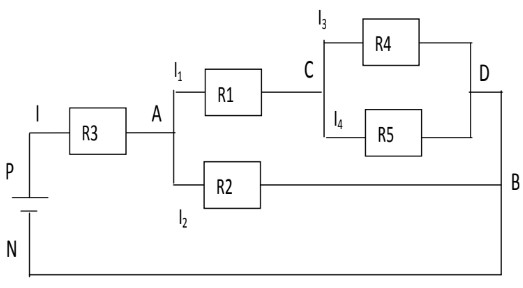
\includegraphics[width=0.5\textwidth]{./img/resistance.png}
\end{center}
\end{document}
